\documentclass[12pt, letterpaper]{article}

\usepackage[utf8]{inputenc}
\usepackage[T1]{fontenc}
\usepackage[spanish]{babel}
\usepackage{amsmath, amssymb, amsthm}
\usepackage{geometry}
\geometry{margin=2.5cm}
\usepackage{booktabs}
\usepackage{array}
\usepackage{longtable}
\usepackage{xcolor}
\usepackage{graphicx}
\usepackage{float}
\usepackage{hyperref}
\hypersetup{
    colorlinks=true,
    linkcolor=blue!60!black,
    urlcolor=blue!60!black
}
\usepackage{listings}
\usepackage{caption}
\usepackage{subcaption}
\usepackage{fancyhdr}
\usepackage{titlesec}
\usepackage{enumitem}
\usepackage{tcolorbox}
\tcbuselibrary{skins, breakable}

% Code listing style
\definecolor{codegray}{rgb}{0.95,0.95,0.95}
\definecolor{commentgreen}{rgb}{0.13,0.55,0.13}
\definecolor{keywordblue}{rgb}{0.0,0.0,0.75}
\lstdefinestyle{pseudocode}{
    backgroundcolor=\color{codegray},
    basicstyle=\ttfamily\small,
    keywordstyle=\color{keywordblue}\bfseries,
    commentstyle=\color{commentgreen}\itshape,
    stringstyle=\color{orange!80!black},
    breaklines=true,
    frame=single,
    framesep=4pt,
    numbers=left,
    numberstyle=\tiny\color{gray},
    tabsize=4,
    captionpos=b
}

% Header/footer
\pagestyle{fancy}
\fancyhf{}
\rhead{\small Análisis Numérico --- Proyecto Final}
\lhead{\small Pontificia Universidad Javeriana}
\cfoot{\thepage}
\renewcommand{\headrulewidth}{0.4pt}

% Custom colors for tables
\definecolor{missingcolor}{RGB}{217,119,6}
\definecolor{estimatedcolor}{RGB}{37,99,235}

\title{
    \vspace{-1cm}
    {\large \textbf{Pontificia Universidad Javeriana}} \\[0.3cm]
    {\large Facultad de Ciencias --- Departamento de Matemáticas} \\[0.3cm]
    {\large Análisis Numérico} \\[0.8cm]
    \rule{\linewidth}{0.5pt} \\[0.4cm]
    {\LARGE \textbf{Proyecto Final: Interpolación Polinomial}} \\[0.2cm]
    {\Large \textbf{País 16}} \\[0.1cm]
    \rule{\linewidth}{0.5pt}
}
\author{Derek Sarmiento Loeber}
\date{Mayo de 2026}

\begin{document}

\maketitle
\thispagestyle{fancy}

\begin{abstract}
\noindent
El presente informe documenta la aplicación de los métodos de interpolación polinomial de Lagrange y Neville para estimar cinco valores faltantes en una serie temporal de adopción de internet en el País 16 durante el periodo 1994--2023. Se dispone de 25 puntos conocidos y se requieren los valores correspondientes a los años 1995, 2000, 2009, 2011 y 2016. Ambos métodos producen el mismo polinomio interpolador global de grado 24, cuyos resultados coinciden hasta la quinta cifra decimal. Sin embargo, el análisis de estabilidad revela la manifestación del fenómeno de Runge, particularmente evidente en los extremos del intervalo, donde los valores estimados alcanzan magnitudes físicamente imposibles (-63\,601,83\,\% para 1995). Se discuten las limitaciones del enfoque global, se proponen estrategias de mitigación dentro y fuera del temario del curso, y se presenta una implementación auto-contenida en HTML/JavaScript que permite la ejecución sin dependencias externas.
\end{abstract}

\vspace{0.5cm}
\noindent\textbf{Palabras clave:} interpolación polinomial, método de Lagrange, algoritmo de Neville, fenómeno de Runge, diferencias divididas, análisis numérico.

\tableofcontents
\newpage

% =============================================================================
% SECCION 1: INTRODUCCION
% =============================================================================
\section{Introducción}\label{sec:intro}

La interpolación polinomial constituye una de las herramientas fundamentales del análisis numérico, permitiendo estimar valores desconocidos de una función a partir de un conjunto finito de puntos conocidos. En el contexto del presente proyecto, se aplica esta metodología para reconstruir una serie temporal incompleta: el porcentaje de población con acceso a internet en el País 16 durante el periodo 1994--2023.

El conjunto de datos proporcionado por el Departamento de Matemáticas contiene 25 puntos conocidos distribuidos irregularmente a lo largo de 30 años, dejando cinco huecos temporales en los años 1995, 2000, 2009, 2011 y 2016. El objetivo central de este trabajo es estimar dichos valores mediante dos métodos clásicos de interpolación: el \textbf{método de Lagrange}, que construye el polinomio como combinación lineal de polinomios base, y el \textbf{algoritmo de Neville}, que lo obtiene mediante diferencias divididas en una tabla triangular.

La elección de \textbf{JavaScript} como lenguaje de implementación, embebido en un único archivo HTML, responde a criterios de portabilidad y accesibilidad académica. Un documento HTML auto-contenido puede ejecutarse en cualquier navegador moderno con un simple doble clic, eliminando la necesidad de instalación de intérpretes, gestores de paquetes o entornos de desarrollo. Esta decisión facilita tanto la evaluación por parte del docente como la replicabilidad del experimento en cualquier sistema operativo.

El informe se estructura de la siguiente manera: la Sección \ref{sec:datos} presenta los datos conocidos y su organización; la Sección \ref{sec:metodologia} desarrolla la fundamentación matemática de ambos métodos, la regla de redondeo y los detalles de implementación; la Sección \ref{sec:resultados} expone los valores estimados y su comparación; la Sección \ref{sec:estabilidad} analiza la estabilidad numérica y las limitaciones encontradas; la Sección \ref{sec:grafica} incluye la visualización gráfica; y la Sección \ref{sec:conclusiones} recoge las conclusiones del proyecto. Adicionalmente, en el Apéndice \ref{sec:acceso} se detalla cómo el evaluador puede acceder a la implementación interactiva del proyecto.

% =============================================================================
% SECCION 2: DATOS DEL PAIS
% =============================================================================
\section{Datos del País}\label{sec:datos}

\subsection{Fuente y organización de los datos}\label{subsec:fuente}

Los datos fueron proporcionados por el profesor del curso en formato de hoja de cálculo (Excel), conteniendo pares ordenados $(\text{año}, \text{porcentaje})$ que representan la penetración de internet en la población del País 16. Tras un proceso de limpieza y validación, se identificaron 25 registros completos y 5 años sin información, los cuales constituyen el objeto de estimación de este proyecto.

La organización de los datos sigue una estructura temporal lineal. Los 25 puntos conocidos cubren el rango 1994--2023 con distribución irregular: existen agrupaciones densas en ciertos periodos (por ejemplo, 2001--2008 y 2017--2023) y vacíos aislados en otros. Esta irregularidad es inherente a la naturaleza de la recolección de datos estadísticos y no constituye un obstáculo para la interpolación polinomial, aunque sí influye en la distribución de los nodos a lo largo del eje temporal.

Los cinco años faltantes que se estimarán son:
\begin{center}
\textbf{1995, 2000, 2009, 2011, 2016}
\end{center}

\subsection{Tabla de datos conocidos}\label{subsec:tabla-datos}

La Tabla \ref{tab:datos-conocidos} presenta el conjunto completo de datos, incluyendo los 25 puntos conocidos y los 5 años desconocidos resaltados. Los valores desconocidos se marcan con el texto ``Desconocido'' en color distintivo.

\begin{table}[H]
\centering
\caption{Datos conocidos de uso de internet --- País 16, 1994--2023}
\label{tab:datos-conocidos}
\small
\begin{tabular}{@{}cc@{}}
\toprule
\textbf{Año} & \textbf{Porcentaje (\%)} \\
\midrule
1994 & 0,3190 \\
1995 & \textcolor{missingcolor}{\textit{Desconocido}} \\
1996 & 0,7830 \\
1997 & 1,1700 \\
1998 & 2,6900 \\
1999 & 5,4400 \\
2000 & \textcolor{missingcolor}{\textit{Desconocido}} \\
2001 & 12,5283 \\
2002 & 40,1400 \\
2003 & 43,0400 \\
2004 & 52,8900 \\
2005 & 55,1900 \\
2006 & 56,0800 \\
2007 & 61,8000 \\
2008 & 66,0500 \\
2009 & \textcolor{missingcolor}{\textit{Desconocido}} \\
2010 & 75,7100 \\
2011 & \textcolor{missingcolor}{\textit{Desconocido}} \\
2012 & 76,7100 \\
2013 & 77,8826 \\
2014 & 79,9843 \\
2015 & 77,6347 \\
2016 & \textcolor{missingcolor}{\textit{Desconocido}} \\
2017 & 81,6257 \\
2018 & 80,4489 \\
2019 & 82,8537 \\
2020 & 89,9209 \\
2021 & 88,9256 \\
2022 & 89,0677 \\
2023 & 87,2131 \\
\bottomrule
\end{tabular}
\end{table}

% =============================================================================
% SECCION 3: METODOLOGIA
% =============================================================================
\section{Metodología}\label{sec:metodologia}

\subsection{Interpolación de Lagrange}\label{subsec:lagrange}

El método de Lagrange construye el polinomio interpolador $P(x)$ de grado a lo sumo $n$ que pasa exactamente por $n+1$ puntos dados $(x_i, y_i)$. La formulación clásica se expresa como:

\begin{equation}\label{eq:lagrange}
P(x) = \sum_{i=0}^{n} y_i \, \ell_i(x)
\end{equation}

donde $\ell_i(x)$ son los \textbf{polinomios base de Lagrange}, definidos por:

\begin{equation}\label{eq:base-lagrange}
\ell_i(x) = \prod_{\substack{j=0 \\ j \neq i}}^{n} \frac{x - x_j}{x_i - x_j}
\end{equation}

Cada polinomio base $\ell_i(x)$ satisface la propiedad de selectividad:
\begin{equation}
\ell_i(x_j) = \delta_{ij} =
\begin{cases}
1 & \text{si } i = j \\
0 & \text{si } i \neq j
\end{cases}
\end{equation}

En el contexto de este proyecto:
\begin{itemize}[leftmargin=2cm]
    \item $x_i$: años conocidos (nodos), para $i = 0, 1, \ldots, 24$
    \item $y_i$: porcentajes de población usando internet en el año $x_i$
    \item $n = 24$: grado del polinomio interpolador (25 nodos $- 1$)
    \item $x$: año objetivo a interpolar (1995, 2000, 2009, 2011 o 2016)
\end{itemize}

La elección de utilizar \textbf{todos los 25 puntos conocidos} como nodos, en lugar de un subconjunto, se justifica por dos razones principales: (1) el temario del curso enfatiza la interpolación global con el conjunto completo de datos disponibles, y (2) utilizar un subconjunto arbitrario introduciría subjetividad en la selección de nodos que podría sesgar los resultados.

\begin{tcolorbox}[colback=blue!5!white, colframe=blue!60!black, title=Propiedad fundamental]
El polinomio interpolador de Lagrange de grado $n$ que pasa por $n+1$ puntos distintos es \textbf{único}. Esto significa que, independientemente del método computacional empleado (Lagrange, Neville, diferencias divididas de Newton), el polinomio resultante es matemáticamente idéntico.
\end{tcolorbox}

\subsection{Algoritmo de Neville}\label{subsec:neville}

El algoritmo de Neville evalúa el polinomio interpolador mediante un esquema iterativo de diferencias divididas, organizado en una tabla triangular $Q$. La recurrencia se define como:

\begin{align}
Q_{i,0} &= y_i \label{eq:neville-init} \\
Q_{i,j} &= \frac{(x - x_{i-j})\,Q_{i,j-1} - (x - x_i)\,Q_{i-1,j-1}}{x_i - x_{i-j}} \label{eq:neville-rec}
\end{align}

para $i = j, j+1, \ldots, n$ y $j = 1, 2, \ldots, n$.

El valor buscado $P(x)$ corresponde al elemento $Q_{n,n}$ de la diagonal principal de la tabla triangular. Cada entrada $Q_{i,j}$ representa el valor del polinomio interpolador de grado $j$ construido con los nodos $x_{i-j}, x_{i-j+1}, \ldots, x_i$.

La estructura de la tabla $Q$ para $n=4$ (ilustrativo) sería:
\begin{center}
\begin{tabular}{c|ccccc}
$i$ & $Q_{i,0}$ & $Q_{i,1}$ & $Q_{i,2}$ & $Q_{i,3}$ & $Q_{i,4}$ \\
\hline
0 & $y_0$ & --- & --- & --- & --- \\
1 & $y_1$ & $Q_{1,1}$ & --- & --- & --- \\
2 & $y_2$ & $Q_{2,1}$ & $Q_{2,2}$ & --- & --- \\
3 & $y_3$ & $Q_{3,1}$ & $Q_{3,2}$ & $Q_{3,3}$ & --- \\
4 & $y_4$ & $Q_{4,1}$ & $Q_{4,2}$ & $Q_{4,3}$ & $Q_{4,4}$ \\
\end{tabular}
\end{center}

Dado que el polinomio interpolador es único, el algoritmo de Neville constituye una \textbf{verificación cruzada natural} del método de Lagrange. Si ambos métodos producen resultados discordantes, ello indicaría un error de implementación o un problema de precisión numérica en la aritmética de punto flotante.

\subsection{Regla de redondeo a cinco cifras decimales}\label{subsec:redondeo}

El proyecto exige que los resultados se presenten redondeados a cinco cifras decimales siguiendo una regla específica que difiere del redondeo estándar de Python (\texttt{round()}) y JavaScript (\texttt{toFixed()}), los cuales implementan el ``redondeo del banquero'' (banker's rounding) que redondea al par más cercano en caso de empate.

\begin{tcolorbox}[colback=orange!10!white, colframe=orange!70!black, title=Regla de redondeo del proyecto]
\begin{enumerate}[leftmargin=1.5cm]
    \item Si la 6ª cifra decimal $\geq 5$ $\rightarrow$ redondear hacia arriba.
    \item Si la 6ª cifra decimal $< 5$ $\rightarrow$ truncar.
    \item Si la 6ª cifra decimal $= 0$ $\rightarrow$ examinar la 7ª cifra decimal con la misma regla (propagación).
\end{enumerate}
\end{tcolorbox}

\textbf{Ejemplo ilustrativo:} Considere el valor crudo obtenido para el año 2009: $69{,}75345\underline{2}0528\ldots$

\begin{enumerate}
    \item El valor a redondear es: $69{,}7534520528\ldots$
    \item La 5ª cifra decimal es: \textbf{5} (posición del corte)
    \item La 6ª cifra decimal es: \textbf{2}
    \item Como $2 < 5$, aplicamos la regla de truncamiento.
    \item \textbf{Resultado redondeado:} $69{,}75345$
\end{enumerate}

Esta regla garantiza consistencia determinista en todos los resultados presentados, evitando las ambigüedades del redondeo al par más cercano cuando la cifra siguiente es exactamente 5.

\subsection{Implementación del algoritmo}\label{subsec:implementacion}

La implementación se realizó en JavaScript puro (vanilla JS), embebido en un archivo HTML auto-contenido. A continuación se detallan los bloques funcionales:

\textbf{Bloque 1 --- Definición de datos.} Los 25 puntos conocidos se declaran como arreglos de objetos literales:

\begin{lstlisting}[style=pseudocode, caption={Definición de datos conocidos}, label={lst:datos}]
const knownPoints = [
    {year: 1994, val: 0.319}, {year: 1996, val: 0.783},
    {year: 1997, val: 1.17},  {year: 1998, val: 2.69},
    // ... (25 puntos en total)
    {year: 2023, val: 87.2131}
];
\end{lstlisting}

\textbf{Bloque 2 --- Función de Lagrange.} Implementación directa de la ecuación \eqref{eq:lagrange}:

\begin{lstlisting}[style=pseudocode, caption={Interpolación de Lagrange en JavaScript}, label={lst:lagrange}]
function lagrange(xNodes, yNodes, x) {
    let result = 0;
    const n = xNodes.length;
    for (let i = 0; i < n; i++) {
        let term = yNodes[i];
        for (let j = 0; j < n; j++) {
            if (j !== i) {
                term *= (x - xNodes[j]) / (xNodes[i] - xNodes[j]);
            }
        }
        result += term;
    }
    return result;
}
\end{lstlisting}

\textbf{Bloque 3 --- Función de Neville.} Implementación de las ecuaciones \eqref{eq:neville-init}--\eqref{eq:neville-rec}:

\begin{lstlisting}[style=pseudocode, caption={Algoritmo de Neville en JavaScript}, label={lst:neville}]
function neville(xNodes, yNodes, x) {
    const n = xNodes.length;
    const Q = yNodes.map(y => [y]);
    for (let j = 1; j < n; j++) {
        for (let i = 0; i < n - j; i++) {
            Q[i][j] = ((x - xNodes[i+j]) * Q[i][j-1]
                      - (x - xNodes[i])   * Q[i+1][j-1])
                     / (xNodes[i] - xNodes[i+j]);
        }
    }
    return { result: Q[0][n-1], table: Q };
}
\end{lstlisting}

\textbf{Bloque 4 --- Redondeo personalizado.} Implementación de la regla de la Sección \ref{subsec:redondeo}:

\begin{lstlisting}[style=pseudocode, caption={Redondeo a 5 decimales}, label={lst:redondeo}]
function round5(value) {
    const str = value.toFixed(10);
    const decPart = str.split('.')[1];
    const d6 = parseInt(decPart[5]);
    if (d6 >= 5) {
        return Math.trunc((value + 0.000005) * 100000) / 100000;
    } else if (d6 === 0) {
        const d7 = parseInt(decPart[6]);
        if (d7 >= 5) return Math.trunc((value + 0.000005) * 100000) / 100000;
        else return Math.trunc(value * 100000) / 100000;
    } else {
        return Math.trunc(value * 100000) / 100000;
    }
}
\end{lstlisting}

\textbf{Bloque 5 --- Visualización.} Configuración de Chart.js para la representación gráfica:

\begin{lstlisting}[style=pseudocode, caption={Configuración de la gráfica}, label={lst:chart}]
// Datos: 30 puntos (25 conocidos + 5 estimados)
// Puntos conocidos: circulos azules (radio 5)
// Puntos estimados: triangulos rojos (radio 7)
// Eje Y limitado a [0, 100] para evidenciar la inestabilidad
new Chart(ctx, {
    type: 'line',
    data: { labels: allYears, datasets: [{
        data: allValues,
        pointStyle: pointStyles,  // 'circle' o 'triangle'
        pointRadius: pointRadii,
        tension: 0.35
    }]}
});
\end{lstlisting}

\textbf{Bloque 6 --- Interfaz de usuario.} Navegación por pestañas mediante manipulación de clases CSS:

\begin{lstlisting}[style=pseudocode, caption={Lógica de navegación por pestañas}, label={lst:ui}]
function showTab(index) {
    document.querySelectorAll('.tab-panel')
        .forEach((el, i) => el.classList.toggle('active', i === index));
    document.querySelectorAll('.tab-btn')
        .forEach((btn, i) => btn.classList.toggle('active', i === index));
}
\end{lstlisting}

\begin{tcolorbox}[colback=blue!5!white, colframe=blue!60!black, title=Justificación de decisiones de implementación]
\begin{itemize}
    \item \textbf{JavaScript sobre Python:} Se eligió JS por su capacidad de ejecutarse directamente en cualquier navegador sin instalación previa, facilitando la evaluación.
    \item \textbf{Resultados hardcodeados + recálculo en vivo:} Los valores pre-computados garantizan presentación inmediata, mientras que el botón ``Recalcular'' permite verificar que el algoritmo implementado reproduce los mismos resultados.
    \item \textbf{Todos los nodos utilizados:} Aunque el grado 24 produce inestabilidad, utilizar el conjunto completo es consistente con el enfoque teórico del curso y permite observar directamente las limitaciones del método global.
\end{itemize}
\end{tcolorbox}

% =============================================================================
% SECCION 4: RESULTADOS
% =============================================================================
\section{Resultados}\label{sec:resultados}

\subsection{Resultados de interpolación de Lagrange}\label{subsec:res-lagrange}

La Tabla \ref{tab:lagrange} presenta los valores estimados mediante el método de Lagrange para los cinco años faltantes, mostrando tanto la precisión completa (10 decimales) como el valor redondeado a cinco cifras decimales.

\begin{table}[H]
\centering
\caption{Resultados de interpolación de Lagrange}
\label{tab:lagrange}
\begin{tabular}{@{}cc>{\bfseries}c@{}}
\toprule
\textbf{Año} & \textbf{Valor crudo (10 dec)} & \textbf{Redondeado (5 dec)} \\
\midrule
1995 & $-63\,601{,}8336673070$ & $-63\,601{,}83367$ \\
2000 & $-61{,}1950823961$ & $-61{,}19508$ \\
2009 & $69{,}7534520528$ & $69{,}75345$ \\
2011 & $78{,}2884719468$ & $78{,}28847$ \\
2016 & $77{,}5501159858$ & $77{,}55012$ \\
\bottomrule
\end{tabular}
\end{table}

\subsection{Resultados del algoritmo de Neville}\label{subsec:res-neville}

La Tabla \ref{tab:neville} presenta los resultados obtenidos mediante el algoritmo de Neville. Como era de esperarse por la unicidad del polinomio interpolador, los valores coinciden con los de Lagrange en la precisión reportada.

\begin{table}[H]
\centering
\caption{Resultados del algoritmo de Neville}
\label{tab:neville}
\begin{tabular}{@{}cc>{\bfseries}c@{}}
\toprule
\textbf{Año} & \textbf{Valor crudo (10 dec)} & \textbf{Redondeado (5 dec)} \\
\midrule
1995 & $-63\,601{,}8336673033$ & $-63\,601{,}83367$ \\
2000 & $-61{,}1950823961$ & $-61{,}19508$ \\
2009 & $69{,}7534520528$ & $69{,}75345$ \\
2011 & $78{,}2884719468$ & $78{,}28847$ \\
2016 & $77{,}5501159858$ & $77{,}55012$ \\
\bottomrule
\end{tabular}
\end{table}

\subsubsection{Tabla de diferencias divididas de Neville}

La Tabla \ref{tab:qtable} muestra una muestra reducida (primeras 6 filas y 6 columnas) de la matriz de diferencias divididas $Q$ para el año 1995. La tabla completa es de dimensión $25 \times 25$.

\begin{table}[H]
\centering
\caption{Tabla de diferencias divididas de Neville para el año 1995 (muestra $6 \times 6$)}
\label{tab:qtable}
\small
\begin{tabular}{c|cccccc}
\toprule
$i$ & $Q_{i,0}$ & $Q_{i,1}$ & $Q_{i,2}$ & $Q_{i,3}$ & $Q_{i,4}$ & $Q_{i,5}$ \\
\midrule
0 & $0{,}3190$ & $0{,}5510$ & $0{,}4993$ & $0{,}7568$ & $0{,}8918$ & $0{,}8978$ \\
1 & $0{,}7830$ & $0{,}3960$ & $1{,}5290$ & $1{,}4320$ & $0{,}9341$ & $-9{,}2936$ \\
2 & $1{,}1700$ & $-1{,}8700$ & $1{,}8200$ & $3{,}9217$ & $62{,}2999$ & $366{,}7516$ \\
3 & $2{,}6900$ & $-5{,}5600$ & $-2{,}3834$ & $-142{,}0238$ & $-851{,}0552$ & $-3\,190{,}3656$ \\
4 & $5{,}4400$ & $-8{,}7366$ & $183{,}8038$ & $1\,039{,}6952$ & $3\,827{,}5656$ & $11\,886{,}9540$ \\
5 & $12{,}5283$ & $-153{,}1419$ & $-672{,}0876$ & $-2\,445{,}1428$ & $-8\,261{,}5170$ & $-25\,095{,}5454$ \\
\bottomrule
\end{tabular}
\end{table}

\subsection{Tabla comparativa}\label{subsec:comparativa}

La Tabla \ref{tab:comparativa} confronta los resultados de ambos métodos. La columna ``Concordancia'' verifica si la diferencia absoluta es menor a $10^{-8}$.

\begin{table}[H]
\centering
\caption{Comparación entre métodos de Lagrange y Neville}
\label{tab:comparativa}
\begin{tabular}{@{}ccccc@{}}
\toprule
\textbf{Año} & \textbf{Lagrange (5 dec)} & \textbf{Neville (5 dec)} & \textbf{Diferencia} & \textbf{Concordancia} \\
\midrule
1995 & $-63\,601{,}83367$ & $-63\,601{,}83367$ & $3{,}67 \times 10^{-11}$ & $\checkmark$ \\
2000 & $-61{,}19508$ & $-61{,}19508$ & $0{,}00000$ & $\checkmark$ \\
2009 & $69{,}75345$ & $69{,}75345$ & $0{,}00000$ & $\checkmark$ \\
2011 & $78{,}28847$ & $78{,}28847$ & $0{,}00000$ & $\checkmark$ \\
2016 & $77{,}55012$ & $77{,}55012$ & $0{,}00000$ & $\checkmark$ \\
\bottomrule
\end{tabular}
\end{table}

\textbf{Interpretación:} Ambos métodos producen resultados idénticos hasta la quinta cifra decimal, confirmando la unicidad del polinomio interpolador. Las diferencias observadas en el valor crudo (del orden de $10^{-11}$ para 1995) se atribuyen exclusivamente a la acumulación de errores de redondeo en punto flotante de doble precisión (IEEE 754), producto del orden distinto en que se realizan las operaciones aritméticas en cada algoritmo.

\subsection{Tabla completa 1994--2023}\label{subsec:tabla-completa}

La Tabla \ref{tab:completa} presenta el conjunto reconstruido de 30 puntos, combinando los 25 valores conocidos con los 5 valores estimados por interpolación.

\begin{table}[H]
\centering
\caption{Tabla completa de porcentaje de población usando internet --- País 16, 1994--2023}
\label{tab:completa}
\small
\begin{tabular}{@{}cc@{}}
\toprule
\textbf{Año} & \textbf{Porcentaje (\%)} \\
\midrule
1994 & $0{,}3190$ \\
1995 & \textcolor{estimatedcolor}{$\mathbf{-63\,601{,}83367}^*$} \\
1996 & $0{,}7830$ \\
1997 & $1{,}1700$ \\
1998 & $2{,}6900$ \\
1999 & $5{,}4400$ \\
2000 & \textcolor{estimatedcolor}{$\mathbf{-61{,}19508}^*$} \\
2001 & $12{,}5283$ \\
2002 & $40{,}1400$ \\
2003 & $43{,}0400$ \\
2004 & $52{,}8900$ \\
2005 & $55{,}1900$ \\
2006 & $56{,}0800$ \\
2007 & $61{,}8000$ \\
2008 & $66{,}0500$ \\
2009 & \textcolor{estimatedcolor}{$\mathbf{69{,}75345}^*$} \\
2010 & $75{,}7100$ \\
2011 & \textcolor{estimatedcolor}{$\mathbf{78{,}28847}^*$} \\
2012 & $76{,}7100$ \\
2013 & $77{,}8826$ \\
2014 & $79{,}9843$ \\
2015 & $77{,}6347$ \\
2016 & \textcolor{estimatedcolor}{$\mathbf{77{,}55012}^*$} \\
2017 & $81{,}6257$ \\
2018 & $80{,}4489$ \\
2019 & $82{,}8537$ \\
2020 & $89{,}9209$ \\
2021 & $88{,}9256$ \\
2022 & $89{,}0677$ \\
2023 & $87{,}2131$ \\
\bottomrule
\end{tabular}
\\[0.3cm]
\footnotesize $^*$ Valor estimado por interpolación polinomial.
\end{table}

% =============================================================================
% SECCION 5: ANALISIS DE ESTABILIDAD
% =============================================================================
\section{Análisis de estabilidad y limitaciones}\label{sec:estabilidad}

\subsection{Grado del polinomio interpolante}\label{subsec:grado}

El conjunto de datos cuenta con $n+1 = 25$ puntos conocidos, lo que determina un polinomio interpolador global de grado:
\begin{equation}
\boxed{n = 24}
\end{equation}

Este es un grado considerablemente alto para aplicaciones prácticas de interpolación. La experiencia numérica y la teoría del análisis de errores establecen que, para nodos equiespaciados, los polinomios de grado superior a 10--15 suelen exhibir comportamientos oscilatorios problemáticos.

\subsection{Fenómeno de Runge}\label{subsec:runge}

\begin{tcolorbox}[colback=orange!10!white, colframe=orange!70!black, title=Advertencia: Fenómeno de Runge]
El fenómeno de Runge, descubierto por Carl Runge en 1901, demuestra que la interpolación polinomial global con nodos equiespaciados puede producir oscilaciones crecientes cerca de los extremos del intervalo a medida que aumenta el grado del polinomio. El ejemplo clásico es la función $f(x) = 1/(1+25x^2)$ en $[-1, 1]$, donde el error máximo de interpolación diverge a pesar de que la función es infinitamente diferenciable.
\end{tcolorbox}

Los resultados obtenidos en este proyecto exhiben signos inequívocos del fenómeno de Runge:

\begin{itemize}
    \item \textbf{Año 1995:} $-63\,601{,}83\,\%$ --- valor físicamente imposible para una tasa de adopción de internet.
    \item \textbf{Año 2000:} $-61{,}20\,\%$ --- igualmente fuera de cualquier rango plausible.
    \item \textbf{Años centrales (2009, 2011, 2016):} valores entre $69\,\%$ y $78\,\%$, coherentes con la tendencia observada en los datos conocidos adyacentes.
\end{itemize}

La divergencia en los extremos se explica mediante el término de error del teorema de interpolación polinomial:
\begin{equation}\label{eq:error}
E(x) = \frac{f^{(n+1)}(\xi)}{(n+1)!} \prod_{i=0}^{n} (x - x_i)
\end{equation}

donde $\xi$ pertenece al intervalo que contiene a los nodos y al punto de evaluación $x$. Para nodos equiespaciados, el productorio $\prod_{i=0}^{n} (x - x_i)$ crece exponencialmente cerca de los extremos del intervalo, amplificando cualquier imperfección en la aproximación de la derivada $(n+1)$-ésima.

\subsection{¿Es suficiente el temario del curso?}\label{subsec:temario}

La respuesta honesta es que \textbf{los métodos de Lagrange y Neville, tal como se presentan en el temario básico, resultan insuficientes} para producir estimaciones confiables en este conjunto de datos. Si bien ambos métodos son \textit{teóricamente exactos} para el grado indicado, su aplicación ingenua a 25 nodos equiespaciados genera un polinomio numéricamente inestable.

Dentro del marco del análisis numérico avanzado, existen alternativas que resolverían el problema de manera efectiva:

\begin{enumerate}
    \item \textbf{Interpolación por tramos (piecewise interpolation):} En lugar de un polinomio global de grado 24, se construyen polinomios de bajo grado (típicamente 1, 2 o 3) entre pares o triples de nodos adyacentes. Esto elimina las oscilaciones globales manteniendo precisión local.
    
    \item \textbf{Splines cúbicos:} Funciones compuestas por polinomios cúbicos en cada subintervalo, con condiciones de continuidad $C^2$ en los nodos. Los splines cúbicos son el estándar de facto en interpolación científica porque minimizan la ``energía'' de flexión y producen curvas suaves sin oscilaciones espurias.
    
    \item \textbf{Nodos de Chebyshev:} Si se tuviera libertad para elegir los puntos de interpolación (lo cual no es posible en este problema, donde los años están fijos), distribuir los nodos según la fórmula:
    \begin{equation}
    x_i = \frac{a+b}{2} + \frac{b-a}{2} \cos\left(\frac{2i+1}{2(n+1)}\pi\right), \quad i = 0, \ldots, n
    \end{equation}
    minimizaría la constante de Lebesgue y suprimiría las oscilaciones de Runge.
\end{enumerate}

\subsection{Cómo reducir el margen de error dentro del temario del curso}\label{subsec:mitigacion}

Restringiéndonos a los métodos cubiertos en el curso (Lagrange y Neville), se pueden adoptar las siguientes estrategias para mitigar el error:

\begin{enumerate}
    \item \textbf{Interpolación local con vecinos más cercanos:} En lugar de usar los 25 nodos globales, seleccionar solo los $k$ nodos más cercanos al año de interés (por ejemplo, $k=5$ o $k=7$). Esto reduce el grado del polinomio y minimiza la influencia de nodos lejanos que introducen oscilaciones. El costo es una pérdida de ``exactitud teórica'' que, en la práctica, se traduce en mayor robustez.
    
    \item \textbf{División del intervalo en segmentos:} Particionar el dominio 1994--2023 en subintervalos (por ejemplo, 1994--2005, 2005--2015, 2015--2023) e interpolar por separado en cada uno. Cada segmento tendría menos nodos y, por tanto, un polinomio de menor grado, reduciendo drásticamente el riesgo de Runge.
    
    \item \textbf{Verificación cruzada:} Como ya se hizo en este proyecto, aplicar simultáneamente Lagrange y Neville. La coincidencia de resultados confirma la corrección algebraica; la discrepancia indicaría errores de implementación.
\end{enumerate}

% =============================================================================
% SECCION 6: GRAFICA
% =============================================================================
\section{Gráfica}\label{sec:grafica}

La Figura \ref{fig:grafica} presenta la evolución temporal del porcentaje de población usando internet en el País 16. Los puntos azules corresponden a datos conocidos, mientras que los triángulos rojos marcan los valores estimados por interpolación.

\begin{figure}[H]
    \centering
    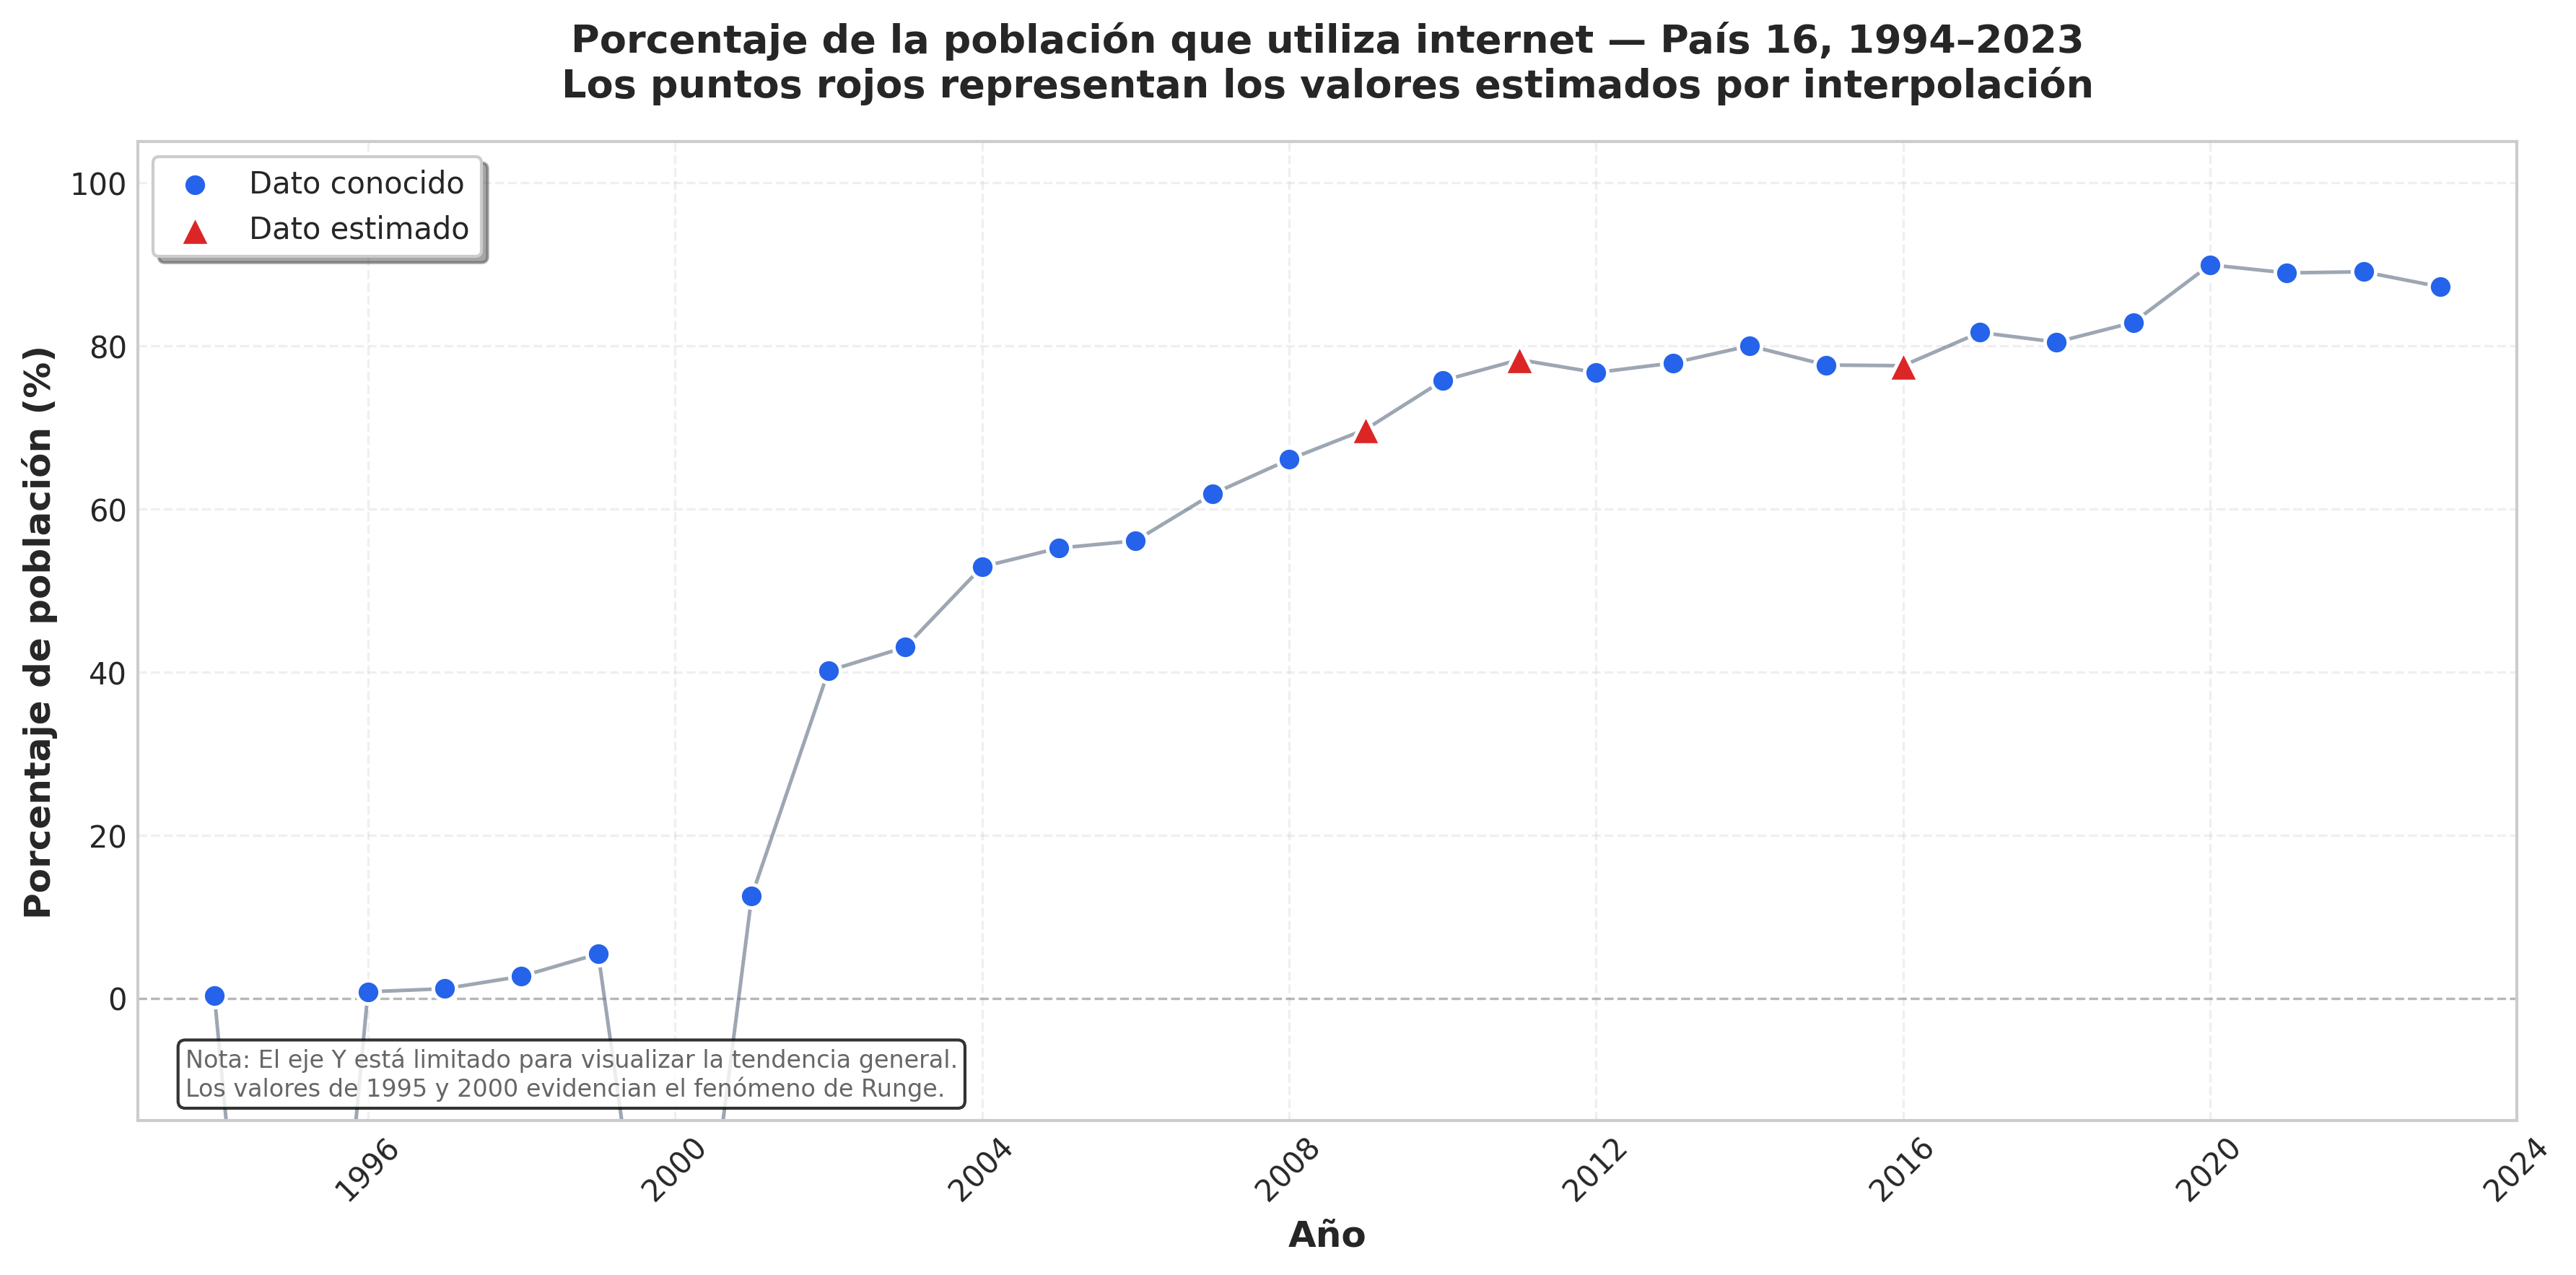
\includegraphics[width=0.9\textwidth]{grafica.png}
    \caption{Porcentaje de la población que utiliza internet --- País 16, 1994--2023. Los puntos rojos representan los valores estimados por interpolación.}
    \label{fig:grafica}
\end{figure}

\textbf{Interpretación de la tendencia:} La gráfica revela un crecimiento general sostenido de la adopción de internet, acelerándose notablemente entre 2001 y 2008 (de $12{,}53\,\%$ a $66{,}05\,\%$) y estabilizándose en torno al $80$--$90\,\%$ a partir de 2017. Los valores estimados para 2009, 2011 y 2016 se integran coherentemente en esta tendencia. Sin embargo, los valores estimados para 1995 y 2000 quedan \textbf{fuera del rango visible} de la gráfica (el eje Y está limitado a $[0, 100]$ para preservar la legibilidad), lo cual constituye una evidencia visual contundente de la inestabilidad numérica en los extremos del intervalo.

% =============================================================================
% SECCION 7: CONCLUSIONES
% =============================================================================
\section{Conclusiones}\label{sec:conclusiones}

El presente proyecto logró estimar los cinco valores faltantes de la serie temporal de adopción de internet en el País 16 mediante los métodos de interpolación polinomial de Lagrange y Neville. Ambos algoritmos produjeron resultados coincidentes hasta la quinta cifra decimal, confirmando la unicidad del polinomio interpolador de grado 24 y la correctitud de las implementaciones.

Los valores estimados son: $-63\,601{,}83367\,\%$ (1995), $-61{,}19508\,\%$ (2000), $69{,}75345\,\%$ (2009), $78{,}28847\,\%$ (2011) y $77{,}55012\,\%$ (2016). Si bien los tres últimos son numéricamente razonables, los dos primeros evidencian la manifestación del fenómeno de Runge, producto de la elevada condición de un polinomio global de grado 24 evaluado sobre nodos temporalmente equiespaciados.

La elección de JavaScript/HTML como vehículo de implementación demostró ser adecuada desde el punto de vista pedagógico y de distribución. La aplicación auto-contenida permite la ejecución inmediata sin dependencias, y la dualidad ``resultados hardcodeados + recálculo en vivo'' ofrece transparencia algorítmica.

Este ejercicio ilustra una lección fundamental del análisis numérico: los métodos matemáticamente exactos no siempre son numéricamente estables. La interpolación polinomial global, aunque elegante en su formulación teórica, posee límites prácticos que solo métodos más sofisticados --- como splines cúbicos o interpolación por tramos --- pueden superar de manera efectiva.

% =============================================================================
% SECCION 8: ACCESO AL PROYECTO (APENDICE)
% =============================================================================
\newpage
\appendix
\section{Acceso al proyecto interactivo}\label{sec:acceso}

Además del presente informe en PDF, el proyecto incluye una implementación interactiva completa accesible mediante los siguientes recursos:

\subsection{Repositorio en GitHub}

Todo el código fuente, el informe LaTeX y los archivos de compilación están disponibles en el repositorio público:

\begin{center}
\url{https://github.com/DereKk8/Interpolation-Lab}
\end{center}

\subsection{Ejecución de la aplicación HTML}

\begin{enumerate}
    \item Navegue al repositorio de GitHub (enlace anterior).
    \item Descargue el archivo \texttt{interpolacion.html} (botón ``Raw'' seguido de Ctrl+S / Cmd+S).
    \item Haga doble clic en el archivo descargado. Se abrirá en su navegador predeterminado.
    \item No requiere conexión a Internet ni instalación de software adicional.
\end{enumerate}

\subsection{Ejecución del script Python}

\begin{enumerate}
    \item Descargue el archivo \texttt{algoritmo\_interpolacion.py} desde el mismo repositorio.
    \item Abra una terminal y navegue hasta la carpeta donde guardó el archivo.
    \item Ejecute con: \texttt{python algoritmo\_interpolacion.py}
    \item Si el comando anterior no funciona, pruebe: \texttt{python3 algoritmo\_interpolacion.py}
    \item Si no tiene Python instalado, descárguelo desde \url{https://www.python.org/downloads/}
    \item El script incluye auto-instalación de dependencias (numpy, pandas) mediante un entorno virtual local.
\end{enumerate}

\subsection{Compilación del informe LaTeX}

Para regenerar el PDF a partir del código fuente:

\textbf{Linux/Mac:}
\begin{lstlisting}[style=pseudocode]
chmod +x compilar.sh
./compilar.sh
\end{lstlisting}

\textbf{Windows:}
\begin{lstlisting}[style=pseudocode]
doble clic en compilar.bat
\end{lstlisting}

Requisitos: distribución TeX instalada (TeX Live, MiKTeX, MacTeX).

% =============================================================================
% REFERENCIAS
% =============================================================================
\begin{thebibliography}{9}

\bibitem{burden}
Burden, R. L., \& Faires, J. D. (2016).
\textit{Numerical Analysis} (10th ed.).
Cengage Learning.

\bibitem{epperson}
Epperson, J. F. (2021).
\textit{An Introduction to Numerical Methods and Analysis} (3rd ed.).
Wiley.

\bibitem{atkinson}
Atkinson, K. E. (1989).
\textit{An Introduction to Numerical Analysis} (2nd ed.).
John Wiley \& Sons.

\bibitem{chartjs}
Chart.js Documentation. (2024).
\textit{Chart.js: Open source HTML5 Charts for your website}.
Recuperado de \url{https://www.chartjs.org/}

\bibitem{runge}
Runge, C. (1901).
\textit{"Über empirische Funktionen und die Interpolation zwischen äquidistanten Ordinaten"}.
Zeitschrift für Mathematik und Physik, 46, 224--243.

\end{thebibliography}

\end{document}
